% kuleuventheme2 by Janez Kren, September 2017, janez.kren@kuleuven.be, based on:
% kuleuventheme 1.3 by Roland Pastorino, 2013 roland.pastorino@kuleuven.be / www.rolandpastorino.com

\documentclass[11pt,t]{beamer}
\usetheme{kuleuven2}	%THEME OPTIONS for LOGO: kul (default), kulak, lrd,    ; OPTIONS for TITLE PAGE: normal (default), sedes
%\usetheme{Ilmenau}

%%% OTHER SETTINGS
\usefonttheme[onlymath]{serif}			% math font with serifs, delete to make it sans-serif
\setbeamertemplate{footline}[body] 		% delete this line to remove footline bar on all frames
%\usepackage[orientation=landscape,size=custom,width=16,height=9,scale=0.5,debug]{beamerposter} %enable for widescreen 16:9 ratio
%\titlegraphic{ \includegraphics[width=.2\paperwidth]{mytitlepagepic.png} } %optional title page image
\newcommand\Fontvi{\fontsize{8}{11}\selectfont}

%%% ADDED PACKAGES:
\usepackage[english]{babel}
\usepackage{amsfonts}
\usepackage{amssymb}
%\setcounter{section}{-1}

\setbeamertemplate{subsection page}
{
    \begingroup
    \begin{beamercolorbox}[sep=2pt,center,rounded=true,shadow=true]{section title}% sep= vertical space around text (between text and box border)
        \usebeamerfont{section title}\insertsection\par
    \end{beamercolorbox}
    \vspace*{-1.pt}%    \vspace*{10pt}
    \begin{beamercolorbox}[sep=6pt,center,rounded=true,shadow=true]{subsection title}
        \usebeamerfont{subsection title}\insertsubsection\par
    \end{beamercolorbox}
    \endgroup
}

\AtBeginSubsection{\frame{\subsectionpage}}

%%% TITLE PAGE INFO:
\title[]{Profiles of tolerance and respect for the rights of \\diverse social groups among youth.} %[]] will appear in footline
\subtitle{Comparisons across countries.}

\author{Pamela Inostroza Fernandez}
\institute{Master in Statistics and Data Science - KU Leuven}
\date{April 2021}




\begin{document}
\csname beamer@calculateheadfoot\endcsname %recalculate head and foot dimension


\begin{frame}[plain,noframenumbering]
	\titlepage
\end{frame}
	

% Table of Contents
\begin{frame}{Table of Contents}
	\hfill	{\large \parbox{.961\textwidth}{\tableofcontents[hideothersubsections]}}
\end{frame}


\section{Introduction}

\begin{frame}[c,plain]{Introduction}
\vspace{-11pt}
International studies such as the International Civic and Citizenship Education Study (ICCS) provides extensive comparative information regarding attitudes among youth.

\vspace{11pt}

Many studies focused on average country comparisons of attitudinal measures based on a variable-centred approach. Focused on the relations among variables and assumes that the sample comes from a homogeneous population, such as Confirmatory Factor Analysis.
\vspace{11pt}

Recent studies started to show the usefulness of person-centred approaches.

\vspace{11pt}

No studies addressed the potential interdependence in these attitudinal dimensions among different subgroups of people.
\end{frame}

\begin{frame}[c,plain]{Research questions}
%\vspace{11pt}

\begin{enumerate}
\item What profiles of attitudes toward diverse groups equality can be distinguished among adolescents in different countries?
\vspace{11pt}

\item Are these profiles comparable across countries?
\vspace{11pt}
\color{lightgray} \item What individual and contextual factors are associated with profile membership? 
\end{enumerate}	
		
\end{frame}

\section{Framework}
\subsection{Mixture models}
\begin{frame}[c,plain]{Mixture models}
\vspace{-11pt}
Is an extension of Generalized Linear Models (GLM), where random as well as fixed effects are allowed in the linear predictor.
\vspace{11pt}

Generalized Linear Mixture Model (GLMM) assumes that some of its parameters differ across unobserved subgroups, latent classes, or mixture components.  
\vspace{11pt}

This is very helpful when we do not know if the population is homogeneous. The mixture of different distributions indicates population heterogeneity.   

\end{frame}


\begin{frame}[c,plain]{Person-centred approach }
\vspace{-11pt}

Clustering tool for categorical variables (similar to k-means clustering for continuous variables).  
Also known as probabilistic cluster analysis.  
\vspace{11pt}

\textbf{Classify respondents into one or more groups (latent classes)}
\vspace{11pt}

\begin{itemize}
\item Identify unobserved subpopulations with similar individuals. 
\item Define a model for the probability of having a response pattern.  
\item Using the probability of belonging to a class, assign individuals to the latent classes. 
\end{itemize}
\end{frame}


\begin{frame}[c,plain]{Latent Class Analysis}
\vspace{-11pt}

A latent class model is a mixture model for a set of categorical items.  
\vspace{11pt}

LCA assumes conditional independence, that the observed categorical indicators are mutually independent once the categorical latent variable is conditioned out.
\vspace{11pt}

\begin{itemize}
\item \textbf{Unconditional probabilities} are latent class probabilities, the proportion of the population expected to belong to a latent class.  
\vspace{2pt}
\item \textbf{Conditional probabilities} are conditional item-response probabilities, measurement parameters, representing the likelihood of endorsing specific characteristics of the observed items, given a specific class membership.
\end{itemize}
		
\end{frame}

\begin{frame}[c,plain]{How identify the number of classes?}
\vspace{-11pt}
An important step in the analysis, different aspects must be considered:
\vspace{11pt}

\begin{itemize}
\item Compare subsequent models by model fit indices.  
\item Evaluate the quality of latent class membership.  
\item Confirm that the size of the latent classes is reasonable.  
\item Identify that the final classes are interpretable based on a theoretical grounding.
\end{itemize}	
\end{frame}

\begin{frame}[c,plain]{Model fit}
\vspace{-11pt}
\begin{itemize}
	\item Akaike's information criterion: 
\begin{itemize}
\item Lower value, tendency to overfit
\end{itemize}	
\item Bayesian information criterion: 
\begin{itemize}
\item Lower value, more severe penalty for complexity
\end{itemize}	
\item Relative entropy: 
\begin{itemize}
\item Perfect classification (entropy = 1)
\end{itemize}	
\item Log-likelihood ratio test (LR, BLRT, Bootstrap\footnotemark)
\begin{itemize}
\item Significant model fit improvement comparing a k-classes and (k-1)-class model
\end{itemize}	

\item Bivariate residuals
\begin{itemize}
\item Residuals values should be close to zero [-1.96 - 1.96]
\end{itemize}

\end{itemize}	

\footnotetext{not available for weighted data}
\end{frame}


\begin{frame}[c,plain]{Multigroup latent class analysis}
\vspace{-11pt}
Measurement invariance can be defined as a conditional independence property of the measurement model with respect to a set of sub-populations within the parent population.  
\vspace{11pt}
\begin{itemize}
\item \textbf{Complete heterogeneous model:} same number of classes but the parameters defining those classes are freely estimated across groups.

\item \textbf{Partial homogeneous model:} equality constraints are imposed across the observed groups, classes are invariant of the group but the size may vary.  

\item \textbf{Complete homogeneous model:}  all parameters are constrained across groups, and the prevalence of latent classes are restricted to be equal across groups.  
\end{itemize}
\end{frame}

\subsection{Large scale assessments}
\begin{frame}[c,plain]{IEA ICCS 2016}

The International Civic and Citizenship Education Study (ICCS)

\begin{itemize}
	\item \textbf{Research:} 
	\begin{itemize}
		\item The way civic and citizenship education is implemented in participating countries
		\item Student's belief about contemporary civic and civic issues in society
	\end{itemize}
	\item \textbf{Population:}  
	\begin{itemize}
		\item more than 94.000 students in 8th grade 
		\item about 3800 schools 
		\item more than 37.000 teachers in those schools
		\item 24 countries
	\end{itemize}
	\item \textbf{Complex sample design:}  stratified two-stage cluster samples
	\begin{itemize}
		\item Schools randomly selected (probability proportional to size)
		\item Intact classrooms sampled at the second stage
	\end{itemize}
	\item \textbf{Complex assessment design:} Booklets, plausible values
\end{itemize}
\end{frame}


\subsection{Methodological features}
\begin{frame}[c,plain]{Methodological features}
\vspace{-11pt}
	\begin{itemize}
		\item \textbf{Exploratory LCA:} No specific hypothesis but the goal is to identify how many classes are necessary to fit the data.  
		\item \textbf{Confirmatory LCA:} Starts with a specific hypothesis, expected frequencies can be estimated and compared with the observed frequencies, if the test indicates that they do not differ significantly the model is appropriate.  
\vspace{11pt}
		\item \textbf{Multigroup LCA:} 	If the measurement properties differ between observed groups (non-invariance), it is not possible to compare the differences between the groups. 
	\end{itemize}
\end{frame}

\subsection{Study}
\begin{frame}[c,plain]{Student's endorsement of equal rights and opportunities}
\vspace{-11pt}
A two dimensional model in a CFA with two scales showed a good fit after controlling for the common residual variance between the negatively worded statements on gender equality\footnotemark.
\footnotetext{ICCS 2016 Technical Report} 
\vspace{5pt}

Level of agreement: ranging from strongly disagree to strongly agree.  
\vspace{5pt}
	\begin{itemize}
		\item \textbf{Attitudes towards gender equality:} Higher values of this scale reflect stronger agreement with the notion of gender equality or stronger disagreement with negative views of gender equality.   
\vspace{11pt}
		\item \textbf{Attitudes towards equal rights for all ethnic/racial groups:} Higher scores indicate a greater degree of agreement with the idea that ethnic and racial groups should have the same rights as other citizens in society.  
	\end{itemize}
\end{frame}


\begin{frame}[c,plain]{Derived scales}
\vspace{5pt}
Two latent dimensions are highly correlated (0.63) and the measurement invariance was within acceptable ranges\footnotemark.  
\vspace{-5pt}
\begin{figure}
\centering
	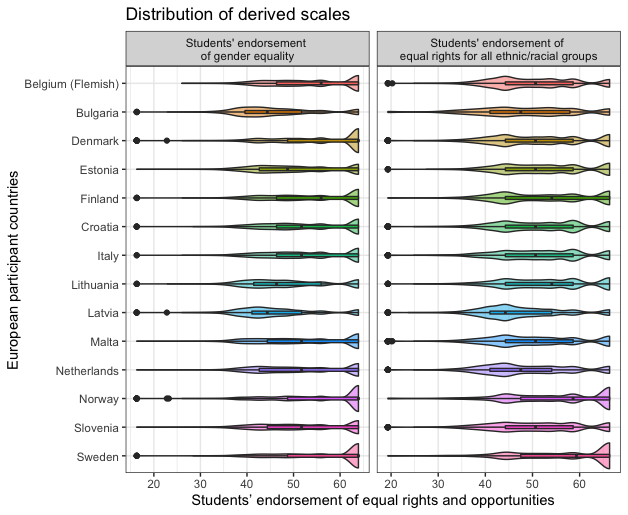
\includegraphics[width=0.7\textwidth]{graphics/derived.png}
\end{figure}	
\footnotetext{ICCS 2016 Technical Report} 

\end{frame}

\section{Methods}
\subsection{Sample}
\begin{frame}{Sample}
\vspace{-5pt}
Students in 8th grade from European participant countries
\small
\begin{center}
\begin{tabular}{l r}
Country & Sample size\\
\hline
Belgium (Flemish) & 2931\\
Bulgaria & 2966\\
Denmark & 6254\\
Estonia & 2857\\
Finland & 3173\\
Croatia & 3896\\
Italy & 3450\\
Lithuania & 3631\\
Latvia & 3224\\
Malta & 3764\\Netherlands & 2812\\
Norway & 6271\\
Slovenia & 2844\\
Sweden & 3264\\
\hline

\end{tabular}
\end{center}
\vspace{3.1mm} 
\end{frame}


\subsection{Variables}
\begin{frame}{Items}
\vspace{5pt}
Level of agreement (dichotomised into agree and disagree).  
\vspace{5pt}
\begin{itemize}
\item \textbf{Attitudes towards gender equality scale}
\vspace{5pt}
	\begin{itemize}
		\item \textbf{GND1:} Men and women should have equal opportunities to take part in government
		\item \textbf{GND2:} Men and women should have the same rights in every way
		\item \textbf{GND5:} Men and women should get equal pay when they are doing the same jobs
		\item \textbf{GND3:} Women should stay out of politics (r)
		\item \textbf{GND4:} Not many jobs available, men should have more right to a job than women (r)
		\item \textbf{GND6:} Men are better qualified to be political leaders than women (r)
	\end{itemize}
\end{itemize}
\end{frame}

\begin{frame}{Items}
\vspace{5pt}
Level of agreement (dichotomised into agree and disagree).  
\vspace{5pt}
\begin{itemize}
\item \textbf{Equal rights for all ethnic and racial groups}
\vspace{5pt}
	\begin{itemize}
		\item \textbf{ETH1:} All ethnic and racial groups should have equal chance to get good education
		\item \textbf{ETH2:} All ethnic and racial groups should have an equal chance to get good jobs
		\item \textbf{ETH3:} All ethnic and racial groups schools should teach students to respect
		\item \textbf{ETH5:} All ethnic and racial groups should have same rights and responsibilities
		\item \textbf{ETH4:} All ethnic and racial groups should be encouraged to run in elections
	\end{itemize}
\end{itemize}
\end{frame}


\subsection{Analytical strategy}
\begin{frame}[c,plain]{Analytical strategy}

\vspace{-11pt}
\begin{enumerate}
\item Independent exploratory LCA to identify country-specific number of classes.
\item Independent analysis to identify country-specific latent class membership, sizes and interpretability.  
\item Identify similar classes across countries.
\item Exploratory LCA with all groups to check if the total number of classes remains.  
\item Evaluate different levels of measurement invariance for the number of comparable classes across countries.
\item Establish a confirmatory analysis with the conditional probabilities and total number of classes identified in the general exploratory LCA model. 
\end{enumerate}
\end{frame}

\section{Results}
\subsection{Attitudes towards gender equality}
\begin{frame}[c,plain]{Independent exploratory LCA by country}
\vspace{-11pt}
	
\begin{figure}
	\centering
	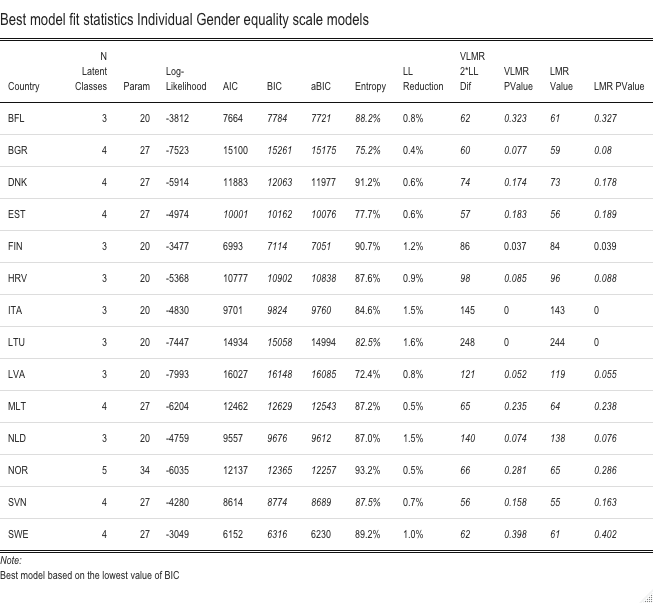
\includegraphics[height=0.7\textwidth]{graphics/countrymodelgender.png}
\end{figure}	
\end{frame} 

\begin{frame}[c,plain]{Independent exploratory LCA by country}
\vspace{-11pt}
	
\begin{figure}
	\centering
	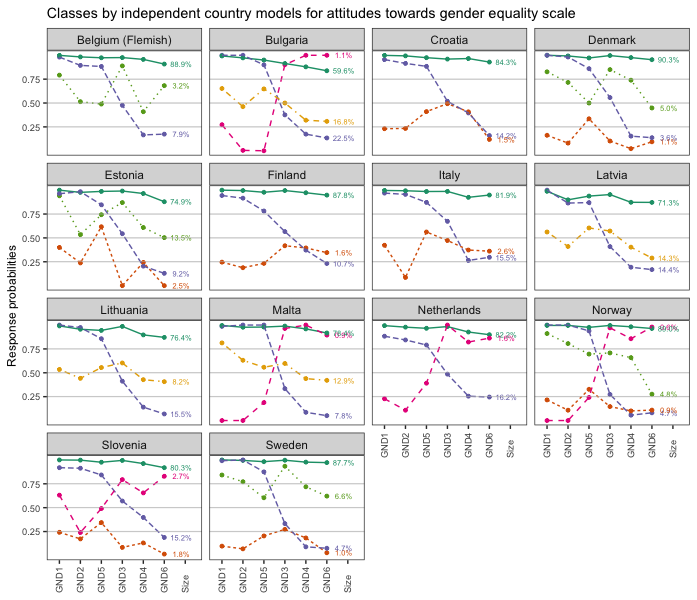
\includegraphics[height=0.7\textwidth]{graphics/ByCntryGender.png}
\end{figure}	
\end{frame} 

\begin{frame}{Classes identified in Attitudes towards gender equality scale}
\vspace{-5pt}

\begin{itemize}
\item \textbf{Fully egalitarian:} Most likely to agree to all items (green line)

\begin{itemize}
	\item Conditional probabilities greater than 0.75 to agree, class sizes around 60\% (Bulgaria) and 90\% (Denmark).  
\end{itemize}
\vspace{5pt}
\item \textbf{Competition-driven sexism:} Most likely to disagree to gender competitive items in favor of women (purple line). 

\begin{itemize}
	\item Conditional probabilities greater than 0.75 to agree to positive views of gender equality and generally lower than 0.5 to agree to reversed negative views, class sizes around 3.6\% (Denmark) and 22.5\% (Bulgaria).  
\end{itemize}
\vspace{5pt}

\item \textbf{Non-egalitarian:} Not likely to agree to any item (orange line)

\begin{itemize}
	\item Conditional probabilities lower to 0.5 to agree to any item, class sizes around 0.9\% (Norway) and 2.6\% (Italy).  
\end{itemize}

\end{itemize}
\end{frame} 


\begin{frame}{Classes identified in Attitudes towards gender equality scale}
\vspace{-5pt}

\begin{itemize}
\item \textbf{Reverse competition-driven sexism:} Most likely to agree to gender competitive items in favor of women (pink line)
\begin{itemize}
	\item Conditional probabilities lower than 0.25 to agree to positive views of gender equality and generally greater than 0.75 to agree to reversed negative views, class sizes around 0.6\% (Norway) and 1.6\% (Netherlands).  
\end{itemize}
\vspace{5pt}
\item \textbf{Political egalitarian:} Likely to agree to political related items (light-green line)

\begin{itemize}
	\item Conditional probabilities greater than 0.75 in political equality items, class sizes around 3.2\% (Belgium) and 1.4\% (Estonia).  
\end{itemize}
\vspace{5pt}
\item \textbf{Random response:} Not defined attitude (yellow line)

\begin{itemize}
	\item Conditional probabilities between 0.25 and 0.75 to agree all items, class sizes around 2.7\% (Slovenia) and 16.8\% (Bulgaria).  
\end{itemize}

\end{itemize}

\end{frame} 

\begin{frame}{Exploratory approach - General model}
	
\begin{figure}
	\centering
	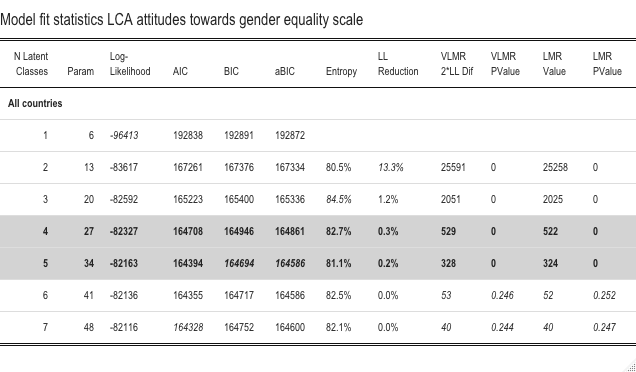
\includegraphics[height=0.5\textwidth]{graphics/modelfitgender.png}
\end{figure}
	
\end{frame} 

\begin{frame}{Best model fit}
	\vspace{-2mm} 
\begin{itemize}
	\item \textbf{AIC}, a 7-class model has the lower value but tendency to overfit suggest to select a lower number of classes model
		\vspace{2mm} 
	\item \textbf{BIC}, considering the penalty for complexity a 5-class model should be selected 
		\vspace{2mm} 
	\item \textbf{Log-likehood ratio test}, a model with 5 classes would indicate a better fit, as the 6-class model do not show a significant improvement in the model fit.
		\vspace{2mm} 
	\item \textbf{Relative entropy}, more than 80\% of the membership is correctly classified based on the model estimated, 3-class has the highest value 84.5\%.
		\vspace{2mm} 
	\item \textbf{Bivariate residuals}, all residuals values in the acceptable range from 5-class model on, just 1 value outside range in the 4-class model. 
\end{itemize}
\end{frame} 



\begin{frame}[c,plain]{Best model fit}
\vspace{-5pt} 
\begin{figure}
	\centering
	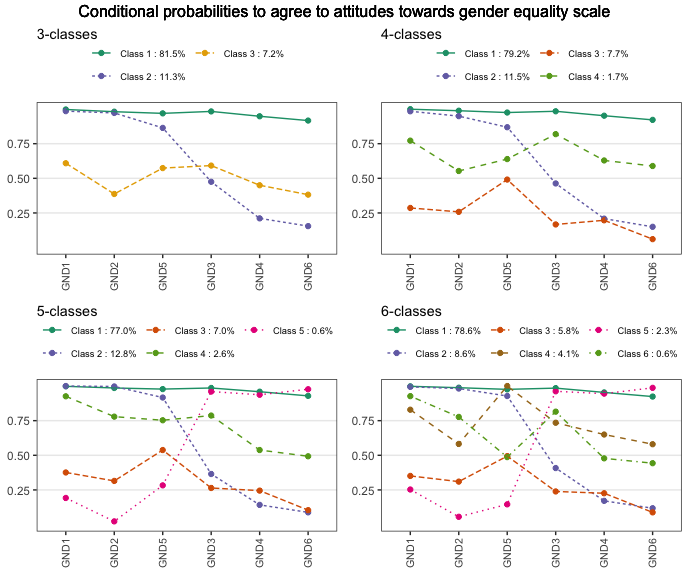
\includegraphics[height=0.7\textwidth]{graphics/genderclasses.png}
\end{figure}

\end{frame} 

\begin{frame}{Profiles identified for comparability}
\begin{itemize}
\item \textbf{3-class model:} 
\begin{enumerate}
	\item Fully egalitarian - ALL COUNTRIES
	\item Competition-driven sexism - ALL COUNTRIES
	\item Random response - BGR, LVA, LTU, MLT
\end{enumerate}
\vspace{3.1mm} 
\item \textbf{4-class model:}  
\begin{enumerate}
	\item Fully egalitarian - ALL COUNTRIES
	\item Competition-driven sexism - ALL COUNTRIES
	\item Non-egalitarian - HRV, DNK, EST, FIN, ITA, NOR, SLV, SWE
	\item Political egalitarian - BFL, DNK, EST, NOR, SWE
\end{enumerate}
\end{itemize}
\end{frame} 

\begin{frame}[c,plain]{Profiles identified for comparability}
\begin{itemize}

\item \textbf{5-class model:}  

\begin{enumerate}
	\item Fully egalitarian - ALL COUNTRIES
	\item Competition-driven sexism - ALL COUNTRIES
	\item Non-egalitarian - HRV, DNK, EST, FIN, ITA, NOR, SLV, SWE
	\item Political egalitarian - BFL, DNK, EST, NOR, SWE
	\item Reverse competition-driven sexism - BGR,  MLT, NLD, NOR, SLV
\end{enumerate}

\vspace{3.1mm} 
\item \textbf{6-class model:}  

\begin{enumerate}
	\item Fully egalitarian - ALL COUNTRIES
	\item Competition-driven sexism - ALL COUNTRIES
	\item Non-egalitarian - HRV, DNK, EST, FIN, ITA, NOR, SLV, SWE
	\item Political egalitarian - BFL, DNK, EST, NOR, SWE
	\item Reverse competition-driven sexism - BGR,  MLT, NLD, NOR, SLV
	\item Pro-women pay/job - Not defined in individual models
\end{enumerate}

\end{itemize}
\end{frame} 

\begin{frame}{Interpretability}
	
\vspace{3.1mm}
\begin{itemize} 
\item With 3 classes: random response class is not very interpretable.

\vspace{3.1mm} 
\item With 6 classes, a new no identified class appears, not interpretable.

\vspace{3.1mm} 
\item With 5 classes, reverse competition-driven sexism class is present in 5 countries but with class sizes lower than 1\%, not representative.


\vspace{3.1mm} 
\item With 4 classes, four main classes are identified across countries.  Two of them are present in all countries. Best model for comparability.
\vspace{3.1mm} 
\item Two remaining classes can be freely estimated that variates in each country and/or with a class size of 0.

\end{itemize}
\end{frame} 

\begin{frame}{Multigroup Latent Class Analysis}

\vspace{-3.1mm} 
\begin{figure}
	\centering
	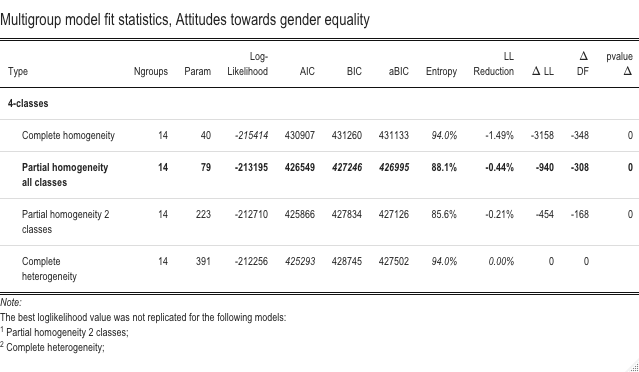
\includegraphics[height=0.5\textwidth]{graphics/MGmodelfitgender.png}
\end{figure}
\end{frame} 

\begin{frame}{Multigroup LCA 4-classes}
\vspace{-3.1mm} 
Partial homogeneity: Conditional probabilities to be equal across countries
\vspace{-3.1mm} 
\begin{figure}
	\centering
	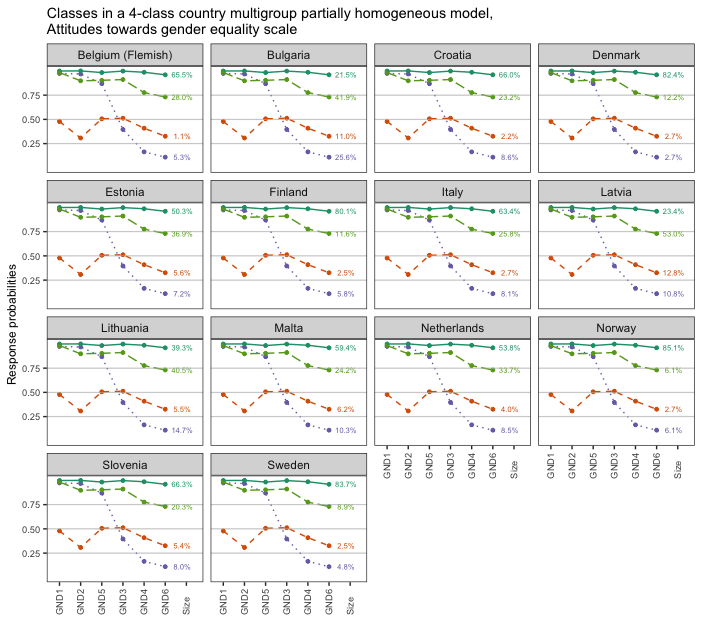
\includegraphics[width=0.6\textwidth]{graphics/MGPHOMgender.png}
\end{figure}
\end{frame} 

%\begin{frame}{Multigroup LCA 4-classes with 2 constrained classes}
%Partially homogeneity: Two classes conditional probabilities constrained to be equal across countries and two classes freely estimated in each country.  
%\begin{figure}
%	\centering
	%\includegraphics[width=0.6\textwidth]{graphics/MGPHOMFixgender.png}
%\end{figure}
%\end{frame} 

%\begin{frame}{Confirmatory approach}
	
%\begin{figure}
%	\centering
%	\includegraphics[width=0.45\textwidth]{graphics/Confgender.png}
%\end{figure}
%\end{frame} 

\subsection{Attitudes towards race and ethnic rights}
\begin{frame}[c,plain]{Independent exploratory LCA by country}
\vspace{-11pt}
	
\begin{figure}
	\centering
	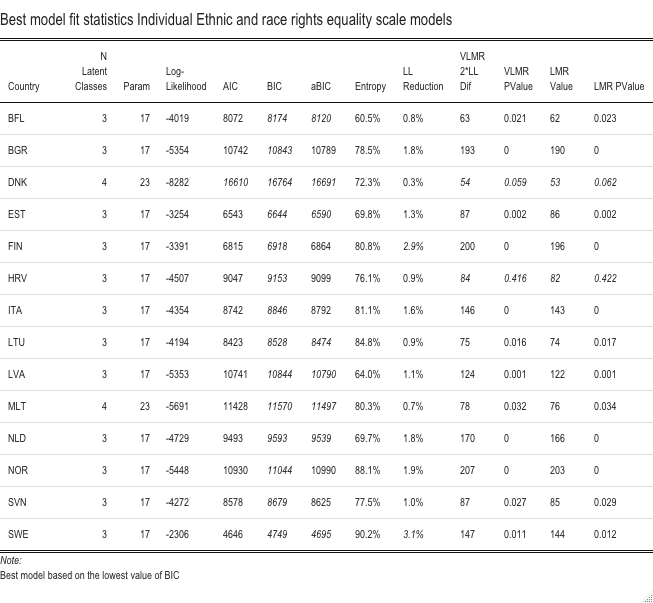
\includegraphics[height=0.7\textwidth]{graphics/countrymodelethnic.png}
\end{figure}	
\end{frame} 

\begin{frame}[c,plain]{Independent exploratory LCA by country}
\vspace{-11pt}
	
\begin{figure}
	\centering
	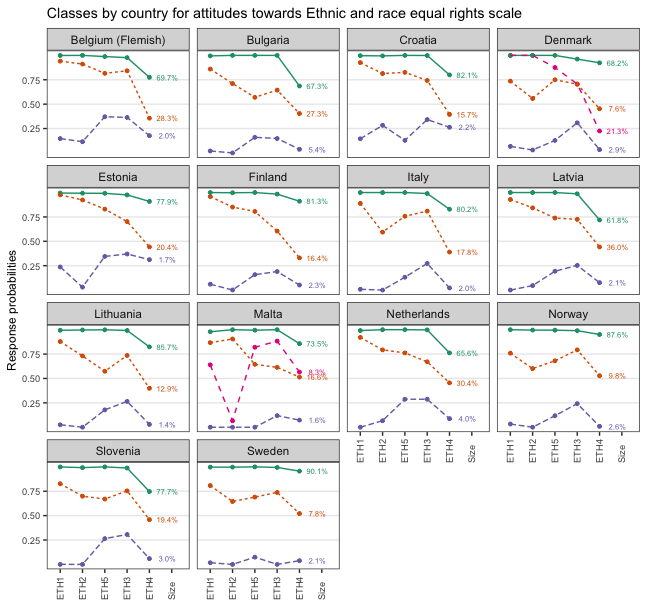
\includegraphics[height=0.7\textwidth]{graphics/ByCntryEthnic.png}
\end{figure}	
\end{frame} 

\begin{frame}[c,plain]{Classes identified - Attitudes towards race and ethnic rights}
\vspace{-5pt}

\begin{itemize}
\item \textbf{Fully egalitarian:}  (green line) 
\begin{itemize}
	\item Conditional probabilities greater than 0.7 to agree, class sizes around 61.8\% (Latvia) and 90\% (Sweden)
\end{itemize}
\vspace{5pt}
\item \textbf{Political non-egalitarian:} (orange line)

\begin{itemize}
	\item Conditional probabilities to agree higher than 0.5 in all items but political item ($< 0.5$), class sizes around 7.6\% (Denmark) and 36\% (Latvia).  
\end{itemize}

\vspace{5pt}
\item \textbf{Non-egalitarian:}  (purple line)

\begin{itemize}
	\item Conditional probabilities lower than 0.5 to agree all items, class sizes around 1.4\% (Lithuania) and 5.4\% (Bulgaria).  
\end{itemize}

\vspace{5pt}
\item \textbf{Country specific class:} (pink line)

\begin{itemize}
	\item Employment non-egalitarian: Class size 8.3\% (Malta)
	\item Strong political non-egalitarian: Class size 21.3\% (Denmark).  
\end{itemize}

\end{itemize}

\end{frame} 

\begin{frame}{Exploratory approach - General model}
	\vspace{-2mm} 
\begin{figure}
	\centering
	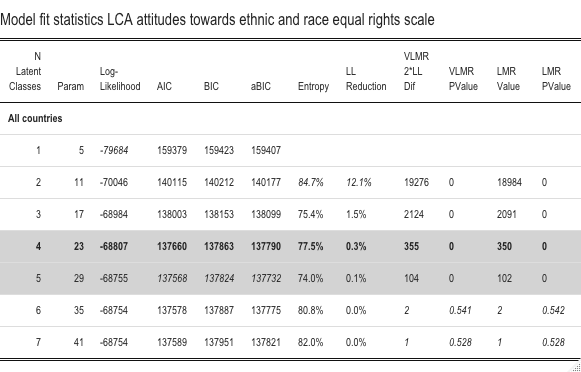
\includegraphics[height=0.5\textwidth]{graphics/modelfitethnic.png}
\end{figure}
	
\end{frame} 

\begin{frame}{Best model fit}

\begin{itemize}
	\item \textbf{AIC}, lower value for the 5-classes model.
	\vspace{2mm} 
	\item \textbf{BIC}, 5-classes considering penalty for complexity.   
	\vspace{2mm} 
	\item \textbf{Log-likehood ratio test}, 5-classes model has better fit compared to the 6-classes model
	\vspace{2mm} 
	\item \textbf{Relative entropy}, 77.5\% is correctly classified in a 4-class model. 
	\vspace{2mm} 
	\item \textbf{Bivariate residuals}, no values out of range from a 4-class model on.
	\end{itemize}
\end{frame} 



\begin{frame}{Best model fit}
\vspace{-5.5mm} 
\begin{figure}
	\centering
	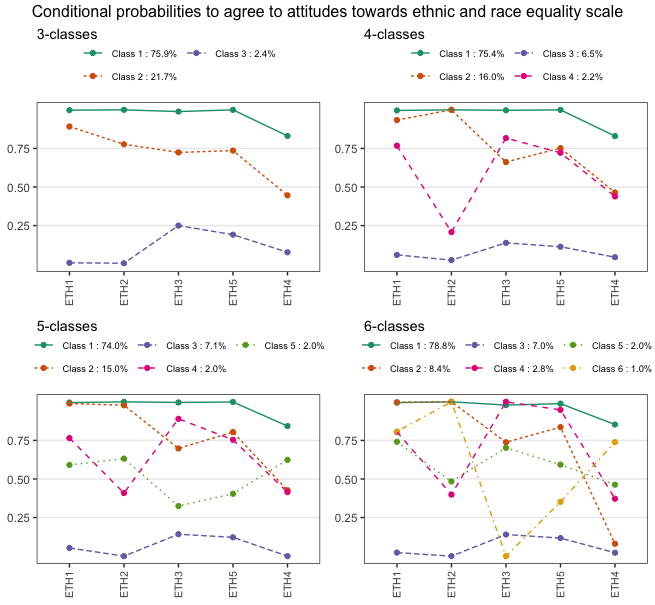
\includegraphics[height=0.63\textwidth]{graphics/ethnicclasses.png}
\end{figure}

\end{frame} 

\begin{frame}[c,plain]{Profiles identified for comparability}
\begin{itemize}
\vspace{-3.1mm} 
\item \textbf{3-class model:} 

\begin{enumerate}
	\item Fully egalitarian: ALL COUNTRIES
	\item Political non-egalitarian: ALL COUNTRIES
	\item Non-egalitarian: ALL COUNTRIES
\end{enumerate}
\vspace{2mm} 

\item \textbf{4-class model:} 

\begin{enumerate}
	\item Fully egalitarian: ALL COUNTRIES
	\item Political non-egalitarian: ALL COUNTRIES
	\item Non-egalitarian: ALL COUNTRIES
	\item Employment non-egalitarian: MLT
\end{enumerate}
\vspace{2mm} 

\item \textbf{5-class model:}  
\begin{enumerate}
	\item Fully egalitarian: ALL COUNTRIES
	\item Political non-egalitarian: ALL COUNTRIES
	\item Non-egalitarian: ALL COUNTRIES
	\item Employment non-egalitarian: MLT
	\item Random response: Not identified in individual models
\end{enumerate}

\end{itemize}
\end{frame} 

\begin{frame}{Interpretability}
	
\begin{itemize}
\item Three main classes found in every model are similar in all countries.

\vspace{3.1mm} 
\item Country specific classes for Malta if more classes are added.

\vspace{3.1mm} 
\item A 4-class model is the better fit to identify three comparable classes and one that variates in each country and/or with size of 0.

\end{itemize}
\end{frame} 

\begin{frame}{Multigroup Latent Class Analysis}
	
\vspace{-3.1mm} 
\begin{figure}
	\centering
	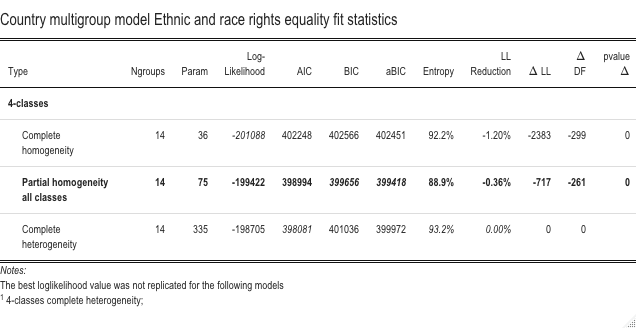
\includegraphics[height=0.5\textwidth]{graphics/MGmodelfitethn.png}
\end{figure}
\end{frame} 

\begin{frame}{Multigroup LCA 4-classes}
\vspace{-3.1mm} 
Partial homogeneity: Conditional probabilities to be equal across countries
\vspace{-3.1mm} 
\begin{figure}
	\centering
	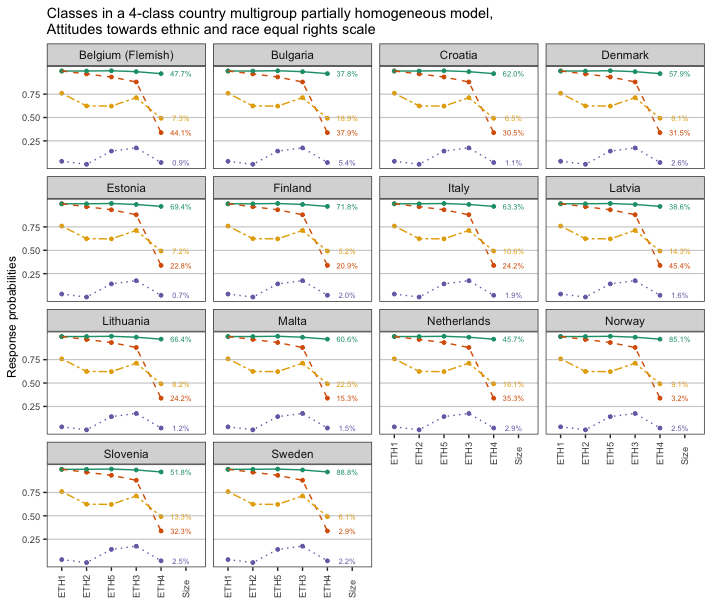
\includegraphics[width=0.6\textwidth]{graphics/MGPHOMethnic.png}
\end{figure}
\end{frame} 

%\begin{frame}{Multigroup LCA 4-classes with 3 constrained classes}
%Partially homogeneity: Three classes conditional probabilities constrained to be equal across countries and one class freely estimated in each country.  
%\begin{figure}
%	\centering
	%\includegraphics[width=0.6\textwidth]{graphics/MGPHOMFixgender.png}
%\end{figure}
%\end{frame} 


%\begin{frame}{Confirmatory approach}
	
%\begin{figure}
%	\centering
%	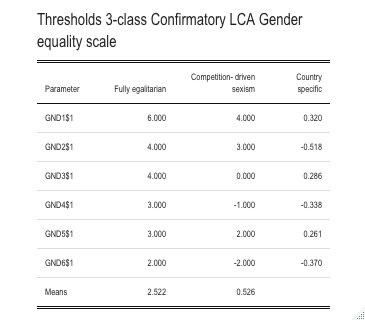
\includegraphics[width=0.45\textwidth]{graphics/thresholdsGender.png}
%	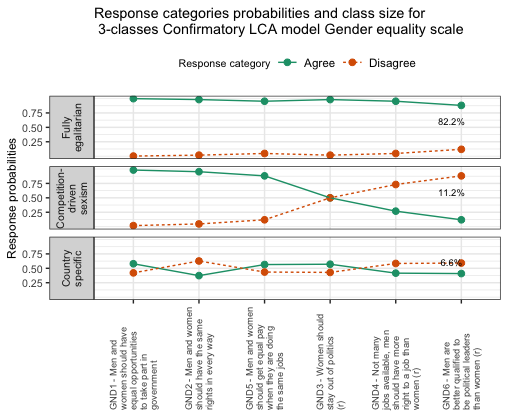
\includegraphics[width=0.45\textwidth]{graphics/ConfGender.png}
%\end{figure}
%\end{frame} 

\section{Conclusion}
\begin{frame}{Conclusions}
\vspace{2mm} 
\begin{itemize}

\item General 
\vspace{2mm} 
\begin{enumerate}
\item Comparability is not assured when we look at subpopulations patterns when analysing Large Scale Assessments.
\vspace{3.1mm} 
\item A independent country analysis is the best strategy to identify common patterns in LSA scales. 
\vspace{3.1mm} 
\item Different country-specific subpopulations were found. 
\vspace{3.1mm} 
\item Some of the patterns are invariants across countries.
\vspace{3.1mm} 
\end{enumerate}
\end{itemize}
\end{frame}

\begin{frame}{Conclusions}
\vspace{-2mm} 
\begin{itemize}

\item Attitudes towards gender equality 
\vspace{2mm} 
\begin{enumerate}
\item Fully egalitarian and Competition-driven sexism are the classes that can be compared across countries. 
\vspace{2mm} 
\item Neighbouring countries can share some patterns. 
\vspace{2mm} 
\item Not clear if there is an impact of inverse worded items in these patterns, the relation with competition-driven sexism class could be forced by wording?.
\end{enumerate}
\vspace{2mm} 
\item Attitudes towards ethnic and race equal rights.  
\vspace{2mm} 
\begin{enumerate}
\item Fully egalitarian, Political non-egalitarian and Non-egalitarian are the classes that can be compared across countries. 
\vspace{2mm} 
\item Not many patterns are identify in every country (3-4).
\end{enumerate}
\end{itemize}
\end{frame}

\section{Further steps?}
\begin{frame}{Further steps?}
\begin{itemize}
\vspace{3.1mm} 
\item Partial homogeneity using conditional probabilities predefined (confirmatory approach) for comparable classes.

\vspace{3.1mm} 
\item Evaluate LCA for all Student’s endorsement of equal rights and opportunities items? (Gender and Ethnic items together) 

\vspace{3.1mm} 
\item Respond to third research question for comparable classes.

\end{itemize}

\end{frame}




\begin{frame}{References}
\Fontvi
\begin{itemize}
\item Agresti, A. (2013). Categorical data analysis (3rd ed).\\

\item Barber, C., \& Ross, J. (2020). Profiles of adolescents’ civic attitudes in sixteen countries\\

\item Davidov, E., Schmidt, P., \& Billiet, J. (Eds.). (2011). Cross-cultural analysis: Methods and applications.\\

\item Hagenaars, J. A., \& McCutcheon, A. L. (Eds.). (2002). Applied latent class analysis (1st ed.). \\

\item Hallquist, M. N., \& Wiley, J. F. (2018). MplusAutomation: An r package for facilitating large-scale latent variable analyses in Mplus. \\

\item Rutkowski, L., Davier, M. von, \& Rutkowski, D. (2014). Handbook of international large-scale assessment background, technical issues, and methods of data analysis.\\

\item Vermunt, J. K. (2014). Latent class model. In A. C. Michalos (Ed.), Encyclopedia of quality of life and well-being research 

\item Wang, J., \& Wang, X. (2020). Structural equation modeling: Applications using mplus (2nd ed.). \\
\end{itemize}
\end{frame} 

\begin{frame}
	\vspace{15mm}
	\begin{center}
Thank you for your feedback!
\end{center}
\end{frame}

\end{document}